\chapter{Gebietsplanung} % (fold)
\label{cha:gebietsplanung}

  \par Ziel: kleine geographische Einheiten (sogenannte Basisgebiete) zu über- geordneten Gebieten (häufig als Bezirke, Cluster oder Territorien bezeichnet) unter der Berücksichtigung verschiedener relevanter Planungskriterien zusammenzufassen.

  \section{Basismodell} % (fold)
  \label{sec:basismodell}

    \subsection{Definitionen und Notationen} % (fold)
    \label{sub:definitionen_und_symbole}

      \par Ein Gebietsplanungsproblem umfasst eine Menge $V = \{1, \dots, M\}$ von Basisgebieten.

    \par Ein \textbf{Basisgebiet} $i \in V$ ist durch seinen Mittelpunkt $b_i = (x_i, y_i)$ bestimmt.

    \par Für jedes Basisgebiet $i \in V$ ist eine einzelne quantifizierbare Eigenschaft, das sogenannte \textbf{Aktivitätsmaß} $w_i$, gegeben. \\

    \par \textbf{Gebiet}:

    \begin{quote}
       \begin{itemize}
          \item Gebiete $D_1, \dots, D_p$ sind disjunkte Teilmengen der Basismenge, so dass jedes Basisgebiet in genau einem Gebiet enthalten ist:
            \begin{equation*}
              D_1 \cup \dots \cup D_p = V \quad \text{und} \quad D_i \cap D_j = \varnothing, i \neq j, b < p
            \end{equation*}
          
          \item Aktivitätsmaß oder die Größe eines Gebiets: die Summe der Aktivitätsmaße seiner Basisgebiete
            \begin{equation*}
              w(D_j) = \sum_{i \in D_j}w_i
            \end{equation*}

          \item \textbf{Zentrum} des Gebiets $j$: $c_j$ (Im Allgemeinen entspricht $c_j$ einem der Mittelpunkte der zum Gebiet $j$ gehörenden Basisgebiete.)
        \end{itemize}
    \end{quote}
     

    \par \textbf{\hl{Zusammenhang}}:

    Basisgebiet $b_i = (x_i, y_i) \in $ Menge der Basisgebiete $V \supseteq$ Gebiet $D_j$
    
    % subsection definitionen_und_symbole (end)

    \subsection{Modell-Kriterien} % (fold)
    \label{sub:modell_kriterien}
      
      \par \textbf{Balance}

      \par Alle Gebiete sollen balanciert sein, also möglichst gleich groß bzw. stark bezüglich der Aktivitätsmaße der Gebiete.

        \begin{quote}
          \begin{itemize}

            \item \textbf{perfekt balnciert} $\Leftrightarrow$ sein Aktivitätsmaß entspricht dem durchschnittlichen Aktivitätsmaß aller Gebiete $\mu$
            \begin{equation}
              \label{mu}
              w(D_j) = \mu = \frac{w(V)}{p}
            \end{equation}

            Auf Grund der diskreten Struktur des Problems können perfekt balancierte Vertriebsgebiete im Allgemeinen NICHT erzielt werden.

            \item \textbf{relative Abweichung} des Aktivitätsmaßes eines Gebiet
            \begin{equation*}
              bal(D_j) = \frac{|w(D_j) - \mu |}{\mu}
            \end{equation*}
          \end{itemize}
        \end{quote}
        

      \par \textbf{Kontiguität (Contiguity)}

      \par Zwei Basisgebiete werden als benachbart bezeichnet, wenn ihre geographischen Anordnungen nichtleere Schnittmengen besitzen.

      \par \textbf{Kompaktheit (Compactness)}

      \begin{quote}
        \begin{itemize}

          \item Reock-Test: Bilde das Verhältnis der Fläche des Gebiets zur Fläche des kleinsten, das Gebiet umschließenden Kreises.
          \begin{equation*}
            cp(D_j) = \frac{A_{A_j}}{A_{uk}} \leq 1
          \end{equation*}

          \begin{figure}[H]
            \centering
            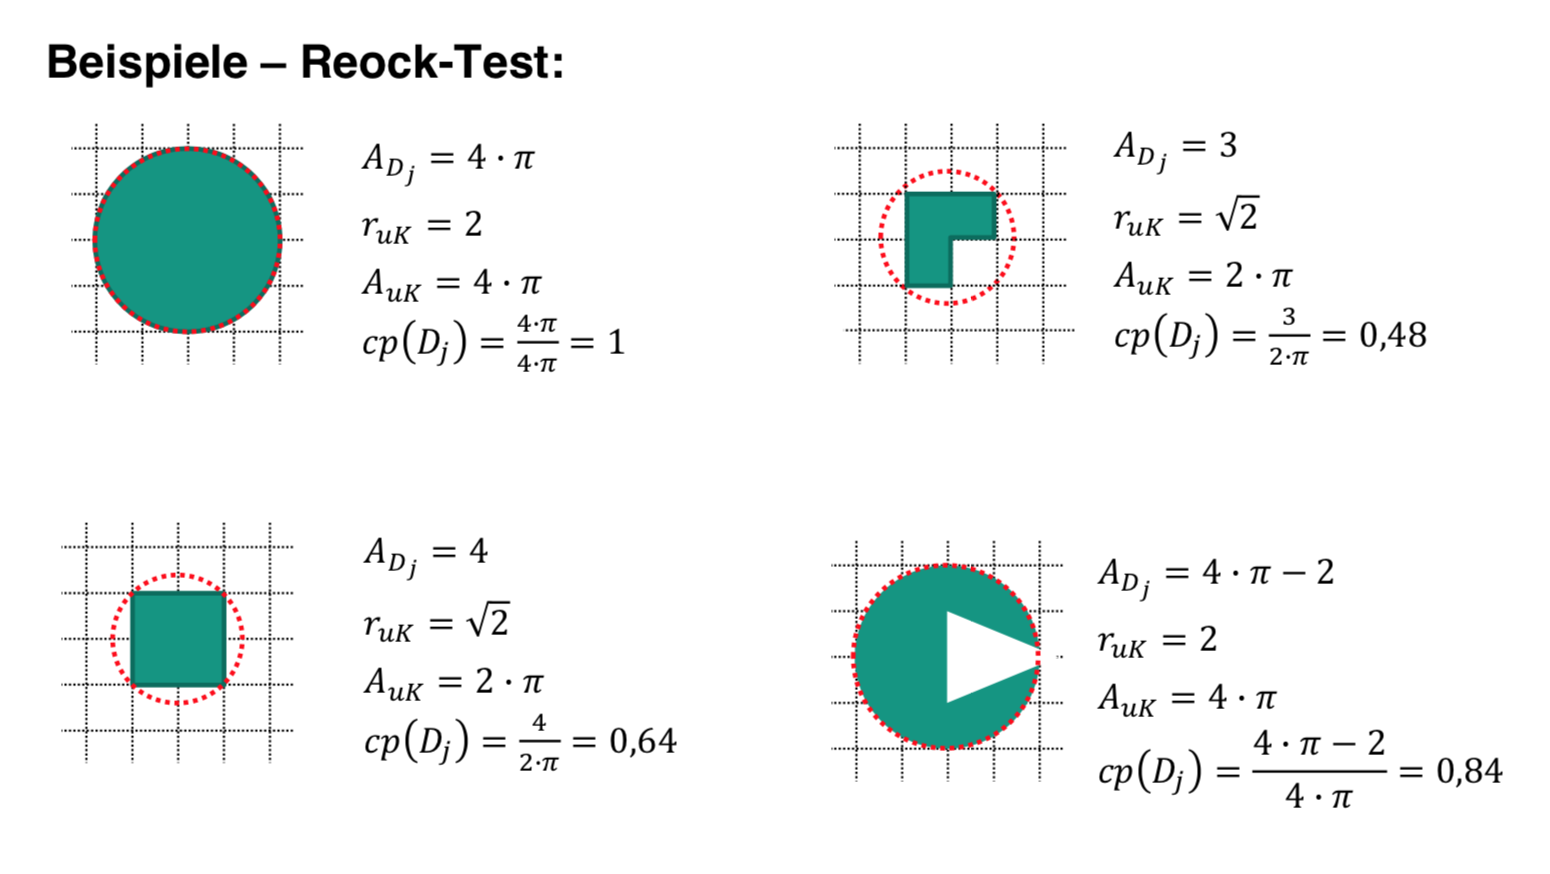
\includegraphics[width=0.95\textwidth]{Images/Reock_Test_Bsp.png}
            \caption{Reock Test Bsp}
            \label{fig:Reock-Test_Bsp}
          \end{figure}

          \item Schwartzberg-Test: Bilde das Verhältnis zwischen dem Umfang eines Kreises, der dadurch festgelegt ist, dass er den gleichen Flächeninhalt wie das Gebiet hat, und dem Umfangs des Gebiets.
          \begin{equation*}
            cp(D_j) = \frac{2 \cdot \sqrt{\pi \cdot A_{D_j}}}{U_{D_j}} \leq 1
          \end{equation*}

          \begin{figure}[H]
            \centering
            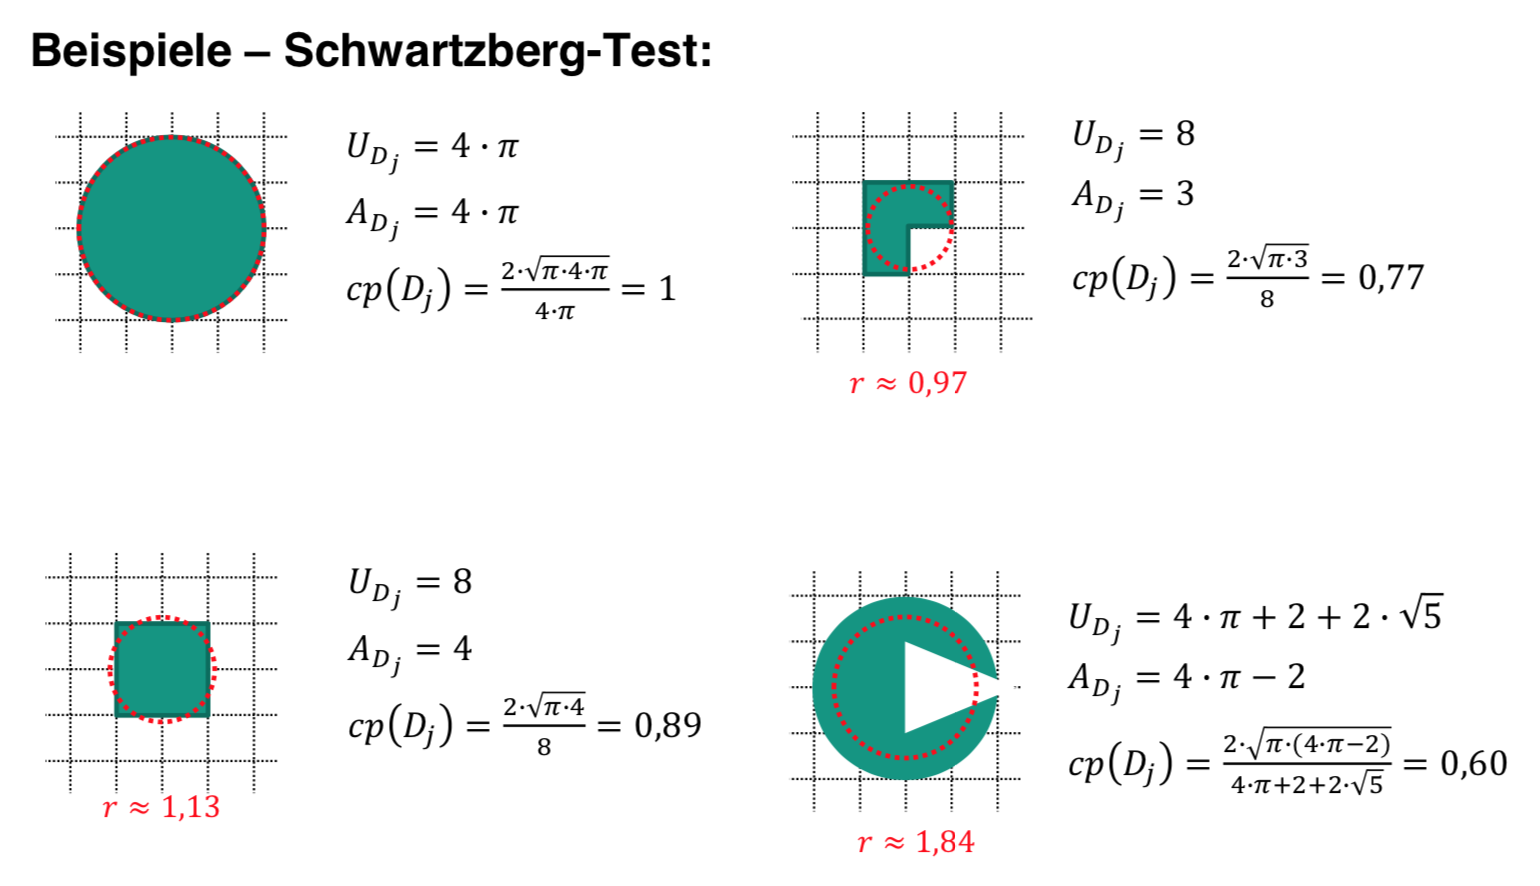
\includegraphics[width=0.95\textwidth]{Images/Schwartzberg_Test_Bsp.png}
            \caption{Schwartzberg-Test Bsp}
            \label{fig:Schwartzberg-Test_Bsp}
          \end{figure}

        \end{itemize}
      \end{quote}
        

        Je näher $cp(D_j)$ an 1, umso kompakter ist das Gebiet.

    % subsection modell_kriterien (end)

    \subsection{Ziel der Gebietsplanung} % (fold)
    \label{sub:ziel_der_gebietsplanung}

      \par Untergliedere alle Basisgebiete $V$ in $p$ Gebiete, welche die Planungskriterien der Balance, Kompaktheit, Kontiguität und Disjunktheit erfüllen.
    
    
    % subsection ziel_der_gebietsplanung (end)
    
  % section basismodell (end)

  \section{Vorgehensweisen zur Gebietsplanung} % (fold)
  \label{sec:vorgehensweisen_zur_gebietsplanung}

    \subsection{Notation} % (fold)
    \label{sub:notation}

      \begin{itemize}
        \item $V$: Menge der Basisgebiete
        \item $w_u$: Aktivitätsmaß des Basisgebiets $u$
        \item $p$: Anzahl der Gebiete
        \item $d_{uv}$: Distanzen
        \item $\mu$: Durchschnittsgröße bzgl. $w$ (\eqref{mu})
        \item $\tau$: Toleranz der Balance
        \item \begin{equation*}
                    x_{uv} = 
                    \begin{cases}
                      1 & \text{falls Basisgebiet } u \text{ einem Gebiet mit dem Zentrum } v \text{ zugeordnet wird.} \\
                      0 & sonst
                    \end{cases}
                \label{trivial wage scheme}
            \end{equation*}
      \end{itemize}
    
    % subsection notation (end)

    \subsection{LP-Formulierung} % (fold)
    \label{sub:lp_formulierung}

      \begin{equation*}
        \begin{aligned}
          & \underset{u,v \in V}{\text{min}}
          & & d_{uv}^2w_{u}x_{uv}\\
          & \text{s.t.}
          & & \sum_{v \in V}x_{uv} = 1 & \quad (u \in V) \quad \text{(Vollst. Zuordnung)}\\ 
          & & & \mu(1 - \tau)x_{vv} \leq \sum_{u \in V}w_ux_{uv} \leq \mu(1 + \tau)x_{vv} &\quad  (v \in V)\quad \quad \text{(Balance)} \\
          & & &\sum_{v \in V}x_{vv} = p \qquad \qquad(p \text{ Gebiete})\\
          & & &x_{uv} \in \{0, 1\}  \qquad (u, v \in V)
        \end{aligned}
        \label{LEN principal problem}
      \end{equation*}
    
    % subsection lp_formulierung (end)
  
  % section vorgehensweisen_zur_gebietsplanung (end)

  \section{Recursive-Partitioning-Algorithmus} % (fold)
  \label{sec:recursive_partitioning_algorithmus}

    \par {\color{blue}{(Bsp: Aufgabe 19)}}

    \par \textbf{Grundidee}:
      \begin{itemize}
         \item Unterteile das Problem rekursiv auf geometrische Weise durch Linien in immer kleinere Teilprobleme.
         \item Wiederhole dies solange, bis eine elementare Größe erreicht ist, in welcher das Gebietsplanungsproblem in effizienter Zeit gelöst wird.
       \end{itemize} 

    \subsection{Definitionen} % (fold)
    \label{sub:definitionen}

      \par \textbf{Partionsproblem}

      \par $PP = (B, q)$ wird als Partitionsproblem bezeichnet, falls $B \subseteq V$ und $1 \leq q \leq p$ gilt.\\
    
      \par \textbf{Linienpartition}

      \par $LP = (B_l, B_r, q_l, q_r)$ wird als Linienpartition bezeichnet, falls:
        \begin{quote}
          \begin{enumerate}
            \item $B_l \cup b_r = B \text{und} B_l \cap B_r = \varnothing$
            \item $\exists \text{ Line } L: B_l = B \cap H^{\leq}(L) \text{ und } B_r = B \cap H^{>}(L)$
            \item $q \leq q_l, q_r \leq q \text{ und } q_l + q_r = q$
          \end{enumerate}
        \end{quote}
    % subsection definitionen (end)   

    \subsection{Recursive-Partitioning} % (fold)
    \label{sub:recursive_partitioning}

      \par \textbf{Gleichmäßige Aufteilung}:

        \begin{quote}
          \begin{itemize}
            \item $q_l = q_r = \frac{q}{2}$, falls $q$ gerade
            \item $q_l = \frac{q - 1}{2}, q_r = \frac{q + 1}{2}$ und $q_l = \frac{q + 1}{2}, q_r = \frac{q - 1}{2}$, falls $q$ ungerade
          \end{itemize}
        \end{quote}

      \par \textbf{Balance}:

      \begin{equation*}
        bal(LP) = \max \{ \frac{|\frac{w(B_L)}{q_l} - \mu|}{\mu}, \frac{|\frac{w(B_r)}{q_r} - \mu|}{\mu}\}
      \end{equation*}

      \par \textbf{Partionsposition}:

      \indent \par Bestimme $k'$, so dass $\frac{w(B_{l}^{k'})}{q_l} < \frac{w(B)}{q}$ und $\frac{w(B_{l}^{k' + 1})}{q_l} \geq \frac{w(B)}{q}$

      \begin{equation*}
        k^* = 
          \begin{cases}
            k' & \text{falls } \frac{w(B)}{q} - \frac{w(B_{l}^{k'})}{q_l} \leq \frac{w(B_{l}^{k' + 1})}{q_l} - \frac{w(B)}{q} \\
            k' + 1 &\text{sonst}
          \end{cases}
      \end{equation*}
    
      \par \textbf{Kompaktheit}:

      \begin{equation*}
        cp(LP) = d(c_1. c_2) = l_2(c_!, c_2)
      \end{equation*}

    % subsection recursive_partitioning (end)

    \subsection{Algorithmus} % (fold)
    \label{sub:algorithmus}

      \par Definiere:

      $$k': \frac{w(B_l^{k'})}{q_l} < \frac{w(B)}{q} \wedge \frac{w(B_l^{k' + 1})}{q_l} \geq \frac{w(B)}{q}$$

      $$
        k^*:= \begin{cases}
          k', & \text{falls } \frac{w(B)}{q} - \frac{w(B_l^{k'})}{q_l} \leq \frac{w(B_l^{k+1})}{q_l} - \frac{w(B)}{q} \\
          k'+1, & sonst
        \end{cases}
      $$


      \begin{algorithm}
        \caption{Recursive-Partitioning-Algorithmus}\label{Recursive-Partitioning-Algorithmus}
        \textbf{Input}: Anzahl Suchrichtungen $K, \beta, V, p$
        \begin{algorithmic}[1]
          % \Procedure{MyProcedure}{}
          \State Markiere Partitionsproblem $PP = (V, p)$ als ungelöst
          \While {es gibt ungelöste Probleme}:
            \State Wähle ein ungelöstes Problem $PP = (B, q)$
            
            \If {$q = 1$}
              \State füge $B$ der Lösungsmenge $DL$ hinzu und markiere $PP$ als gelöst
            \EndIf

            \If {$q > 1$}
              \State Bestimme für jede Suchrichtung die Linienpartition $LP(k^*)$ mit der besten Balance

              $$bal(LP) = max\{\frac{|\frac{w(B_l)}{q_l} - \mu|}{\mu}, \frac{|\frac{w(B_r)}{q_r} - \mu|}{\mu}\}$$

              und füge sie einer Menge $FLP$ hinzu.
              \State Bewerte alle Linienpartitionen $LP$ der Menge $FLP$ durch:
              
                \begin{equation*}
                  rk(LP) = \beta\frac{bal(LP)}{bal^{max}} + (1 - \beta)\frac{cp(LP)}{cp^{max}}
                \end{equation*}
              mit 
              $$cp(LP) = d(c_1, c_2) = l_2(c_1, c_2)$$
              \State Wähle $LP^{*} = (B_{l}^{*}, B_{r}^{*}, q_{l}^{*}, q_{r}^{*}) = \underset{LP \in FLP}{\text{min}}rk(FLP)$ 

              \State Erstelle Partitionsprobleme $PP_l = (B_{l}^{*}, q_{l}^{*})$ und $PP_r = (B_{r}^{*}, q_{r}^{*})$ und markiere sie als ungelöst, markiere $PP$ als gelöst.
            \EndIf
          \EndWhile
          % \EndProcedure
        \end{algorithmic}
        \textbf{Output:} Gebietslayout DL
      \end{algorithm}


    
    % subsection algorithmus (end)
        
       
  % section recursive_partitioning_algorithmus (end)


% chapter gebietsplanung (end)




    


